
%{{第三十二回}}{第三十二回}}

\chapter{诉肺腑心迷活宝玉 含耻辱情烈死金钏}\label{part0036_split_000.htmlux5cux23calibre_pb_0}

{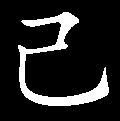
\includegraphics[width=3mm]{../Images/00003}前明显祖汤先生有怀人诗一绝,读之堪合此回,故录之以待知音:}

{无情无尽却情多,情到无多得尽么?}

{解到多情情尽处,月中无树影无波。}\href{../Text/part0036_split_000.html\#lnkback_1_a}{\textsuperscript{①}}

话说宝玉见那麒麟,心中甚是欢喜,便伸手来拿,笑道:``亏你拣着了。你是那里拣的?''史湘云笑道:``幸而是这个,明儿倘或把印也丢了,难道也就罢了不成?''宝玉笑道:``倒是丢了印平常,若丢了这个,我就该死了。''

袭人斟了茶来与史湘云吃,一面笑道:``大姑娘,听见前儿你大喜了。''史湘云红了脸,吃茶不答。袭人道:``这会子又害臊了。你还记得十年前,咱们在西边暖阁住着,晚上你同我说的话儿?那会子不害臊,这会子怎么又害臊了?''史湘云笑道:``你还说呢。那会子咱们那么好。后来我们太太没了,我家去住了一程子,怎么就把你派了跟二哥哥,我来了,你就不像先待我了。''袭人笑道:``你还说呢。先姐姐长姐姐短哄着我替你梳头洗脸,作这个弄那个,{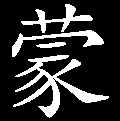
\includegraphics[width=3mm]{../Images/00006}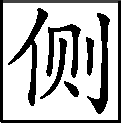
\includegraphics[width=3mm]{../Images/00011}\footnotesize \kaishu 大家风范,情景逼真。}如今大了,就拿出小姐的款来。你既拿小姐的款,我怎敢亲近呢?''史湘云道:``阿弥陀佛,冤枉冤哉!我要这样,就立刻死了。你瞧瞧,这么大热天,我来了,必定赶来先瞧瞧你。不信你问问缕儿,我在家时时刻刻那一回不念你几声。''话未了,忙的袭人和宝玉都劝道:``顽话你又认真了。还是这么性急。''史湘云道:``你不说你的话噎人,倒说人性急。''一面说,一面打开手帕子,将戒指递与袭人。{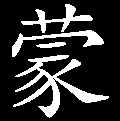
\includegraphics[width=3mm]{../Images/00006}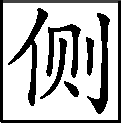
\includegraphics[width=3mm]{../Images/00011}\footnotesize \kaishu 心中意中,多少情致。}

袭人感谢不尽,因笑道:``你前儿送你姐姐们的,我已得了;今儿你亲自又送来,可见是没忘了我。只这个就试出你来了。戒指儿能值多少,可见你的心真。''史湘云道:``是谁给你的?''袭人道:``是宝姑娘给我的。''湘云笑道:``我只当是林姐姐给你的,原来是宝钗姐姐给了你。我天天在家里想着,这些姐姐们再没一个比宝姐姐好的。可惜我们不是一个娘养的。{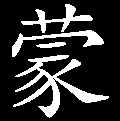
\includegraphics[width=3mm]{../Images/00006}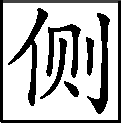
\includegraphics[width=3mm]{../Images/00011}\footnotesize \kaishu 感知己之一叹。}我但凡有这么个亲姐姐,就是没了父母,也是没妨碍的。''说着,眼睛圈儿就红了。{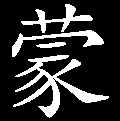
\includegraphics[width=3mm]{../Images/00006}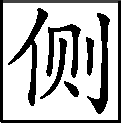
\includegraphics[width=3mm]{../Images/00011}\footnotesize \kaishu 千古同慨。}宝玉道:``罢,罢,罢!不用提这个话。''史湘云道:``提这个便怎么?我知道你的心病,恐怕你的林妹妹听见,又怪嗔我赞了宝姐姐。可是为这个不是?''袭人在旁``嗤''的一笑,说道:``云姑娘,你如今大了,越发心直口快了。''宝玉笑道:``我说你们这几个人难说话,果然不错。''史湘云道:``好哥哥,你不必说话教我恶心。只会在我们跟前说话,见了你林妹妹,又不知怎么了。''{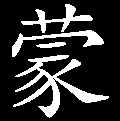
\includegraphics[width=3mm]{../Images/00006}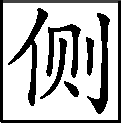
\includegraphics[width=3mm]{../Images/00011}\footnotesize \kaishu 豪爽情形如画。}

袭人道:``且别说顽话,正有一件事还要求你呢。''史湘云便问:``什么事?''袭人道:``有一双鞋,抠了垫心子。我这两日身上不好,不得做,你可有工夫替我做做?''史湘云笑道:``这又奇了,你家放着这些巧人不算,还有什么针线上的,裁剪上的,怎么教我做起来?你的活计叫谁做,谁好意思不做呢。''袭人笑道:``你又糊涂了。你难道不知道,我们这屋里的针线,{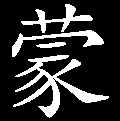
\includegraphics[width=3mm]{../Images/00006}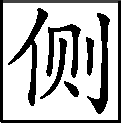
\includegraphics[width=3mm]{../Images/00011}\footnotesize \kaishu ``我们这屋里''等字,精神活跳。}是不要那些针线上的人做的。''史湘云听了,便知是宝玉的鞋了,因笑道:``既这么说,我就替你做了罢。只是一件,你的我才作,别人的我可不能。''袭人笑道:``又来了,我是个什么,就烦你做鞋了。实告诉你,可不是我的。你别管是谁的,横竖我领情就是了。''史湘云道:``论理,你的东西也不知烦我做了多少了,今儿我倒不做了的原故,你必定也知道。''袭人道:``倒也不知道。''{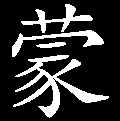
\includegraphics[width=3mm]{../Images/00006}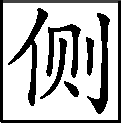
\includegraphics[width=3mm]{../Images/00011}\footnotesize \kaishu 反衬叠起,灵活之至。}史湘云冷笑道:``前儿我听见把我做的扇套子拿着和人家比,赌气又铰了。我早就听见了,你还瞒我。这会子又叫我做,我成了你们的奴才了。''宝玉忙笑道:``前儿的那事,本不知是你做的。''袭人也笑道:``他本不知是你做的。是我哄他的话,说是新近外头有个会做活的女孩子,说扎的出奇的花,我叫他拿了一个扇套子试试看好不好。他就信了,拿出去给这个瞧给那个看的。不知怎么又惹恼了林姑娘,铰了两段。回来他还叫赶着做去,我才说了是你作的,他后悔的什么似的。''{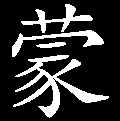
\includegraphics[width=3mm]{../Images/00006}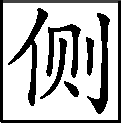
\includegraphics[width=3mm]{../Images/00011}\footnotesize \kaishu 描神!}史湘云道:``越发奇了。林姑娘他也犯不上生气,他既会剪,就叫他做。''袭人道:``他可不作呢。饶这么着,老太太还怕他劳碌着了。大夫又说好生静养才好,谁还烦他做?旧年好一年的工夫,做了个香袋儿;今年半年,还没见拿针线呢。''

正说着,有人来回说:``兴隆街的大爷来了,老爷叫二爷出去会。''宝玉听了,便知是贾雨村来了,心中好不自在。袭人忙去拿衣服。宝玉一面蹬着靴子,一面抱怨道:``有老爷和他坐着就罢了,{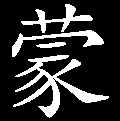
\includegraphics[width=3mm]{../Images/00006}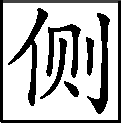
\includegraphics[width=3mm]{../Images/00011}\footnotesize \kaishu 原本烦俗。}回回定要见我。''史湘云一边摇着扇子,笑道:``自然你能会宾接客,老爷才叫你出去呢。''宝玉道:``那里是老爷,都是他自己要请我去见的。''湘云笑道:``主雅客来勤,自然你有些警他的好处,他才只要会你。''宝玉道:``罢,罢,我也不敢称雅,俗中又俗的一个俗人,并不愿同这些人往来。''{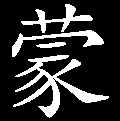
\includegraphics[width=3mm]{../Images/00006}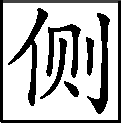
\includegraphics[width=3mm]{../Images/00011}\footnotesize \kaishu 我也不知宝玉是雅是俗,请诸同类一拟。}

湘云笑道:``还是这个情性不改。如今大了,你就不愿读书去考举人进士的,也该常常的会会这些为官做宰的人们,谈谈讲讲些仕途经济的学问,也好将来应酬世务,日后也有个朋友。没见你成年家只在我们队里搅些什么!''宝玉听了道:``姑娘请别的姊妹屋里坐坐,我这里仔细污了你知经济学问的。''袭人道:``云姑娘快别说这话。{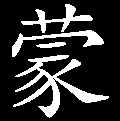
\includegraphics[width=3mm]{../Images/00006}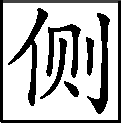
\includegraphics[width=3mm]{../Images/00011}\footnotesize \kaishu 此际不同湘云一语,湘云也实难出一语。}上回也是宝姑娘也说过一回,他也不管人脸上过的去过不去,他就``咳''了一声,拿起脚来走了。这里宝姑娘的话也没说完,见他走了,登时羞的脸通红,说又不是,不说又不是。幸而是宝姑娘,那要是林姑娘,不知又闹到怎么样,哭的怎么样呢。提起这个话来,真真的宝姑娘叫人敬重,自己讪了一会子去了。我倒过不去,{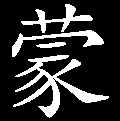
\includegraphics[width=3mm]{../Images/00006}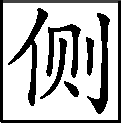
\includegraphics[width=3mm]{../Images/00011}\footnotesize \kaishu 袭人善解忿。}只当他恼了。谁知过后还是照旧一样,真真有涵养,心地宽大。谁知这一个反倒同他生分了。那林姑娘见你赌气不理他,你得赔多少不是呢。''宝玉道:``林姑娘从来说过这些混帐话不曾?若他也说过这些混帐话,我早和他生分了。''{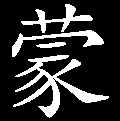
\includegraphics[width=3mm]{../Images/00006}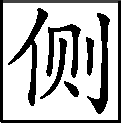
\includegraphics[width=3mm]{../Images/00011}\footnotesize \kaishu 花爱水清明,水怜花色鲜。浮落虽同流,空惹鱼龙涎。}袭人和湘云都点头笑道:``这原是混帐话。''{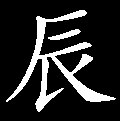
\includegraphics[width=3mm]{../Images/00009}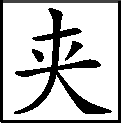
\includegraphics[width=3mm]{../Images/00012}\footnotesize \kaishu 写足!憨宝玉殊可发一大笑。}

原来林黛玉知道史湘云在这里,宝玉一定又赶来说麒麟的原故。因此心下忖度着,近日宝玉弄来的外传野史,多半才子佳人都因小巧玩物上撮合,或有鸳鸯,或有凤凰,或玉环金佩,或鲛帕鸾绦,皆由小物而遂终身。今忽见宝玉亦有麒麟,便恐借此生隙,同史湘云也做出那些风流佳事来。因而悄悄走来,见机行事,以察二人之意。不想刚走来,正听见史湘云说经济一事,宝玉又说:``林妹妹不说这样混帐话,若说这话,我也和他生分了。''林黛玉听了这话,不觉又喜又惊,又悲又叹。所喜者,果然自己眼力不错,素日认他是个知己,果然是个知己。所惊者,他在人前一片私心称扬于我,其亲热厚密,竟不避嫌疑。所叹者,你既为我之知己,自然我亦可为你之知己矣;既你我为知己,则又何必有金玉之论哉;既有金玉之论,亦该你我有之,则又何必来一宝钗哉!所悲者,父母早逝,虽有铭心刻骨之言,无人为我主张。况近日每觉神思恍惚,病已渐成,医者更云气弱血亏,恐致劳怯之症。你我虽为知己,但恐自不能久待;你纵为我知己,奈我薄命何!想到此间,不禁滚下泪来。{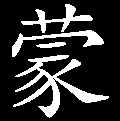
\includegraphics[width=3mm]{../Images/00006}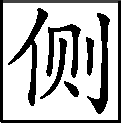
\includegraphics[width=3mm]{../Images/00011}\footnotesize \kaishu 普天下才子佳人、英雄侠{[}士{]}都同来一哭!我虽愚浊,也愿同声一哭。}待进去相见,自觉无味,便一面拭泪,一面抽身回去了。

这里宝玉忙忙的穿了衣裳出来,忽见林黛玉在前面慢慢的走着,似有拭泪之状,便忙赶上来,{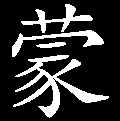
\includegraphics[width=3mm]{../Images/00006}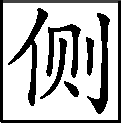
\includegraphics[width=3mm]{../Images/00011}\footnotesize \kaishu 关心情致。}笑道:``妹妹往那里去?怎么又哭了?又是谁得罪了你?''林黛玉回头见是宝玉,便勉强笑道:``好好的,我何曾哭了。''宝玉笑道:``你瞧瞧,眼睛上的泪珠儿未干,还撒谎呢。''一面说,一面禁不住抬起手来替他拭泪。林黛玉忙向后退了几步,说道:``你又要死了!{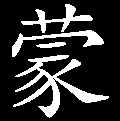
\includegraphics[width=3mm]{../Images/00006}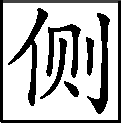
\includegraphics[width=3mm]{../Images/00011}\footnotesize \kaishu 娇羞态!}作什么这么动手动脚的!''宝玉笑道:``说话忘了情,不觉的动了手,也就顾不的死活。''林黛玉道:``你死了倒不值什么,只是丢下了什么金,又是什么麒麟,可怎么样呢?''一句话又把宝玉说急了,赶上来问道:``你还说这话,到底是咒我还是气我呢?''林黛玉见问,方想起前日的事来,遂自悔自己又说造次了,忙笑道:``你别着急,我原说错了。这有什么的,筋都暴起来,急的一脸汗。''一面说,一面禁不住近前伸手替他拭面上的汗{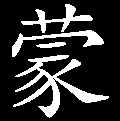
\includegraphics[width=3mm]{../Images/00006}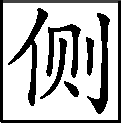
\includegraphics[width=3mm]{../Images/00011}\footnotesize \kaishu 痴情态。}。

宝玉瞅了半天,方说道``你放心''三个字。{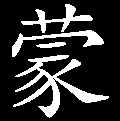
\includegraphics[width=3mm]{../Images/00006}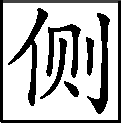
\includegraphics[width=3mm]{../Images/00011}\footnotesize \kaishu 连我今日看之也不懂.是何等文章!}林黛玉听了,怔了半天,方说道:``我有什么不放心的?我不明白这话。你倒说说怎么放心不放心?''宝玉叹了一口气,问道:``你果不明白这话?难道我素日在你身上的心都用错了?连你的意思若体贴不着,就难怪你天天为我生气了。''林黛玉道:``果然我不明白放心不放心的话。''宝玉点头叹道:``好妹妹,你别哄我。果然不明白这话,不但我素日之意白用了,且连你素日待我之意也都辜负了。{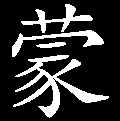
\includegraphics[width=3mm]{../Images/00006}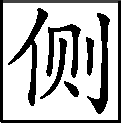
\includegraphics[width=3mm]{../Images/00011}\footnotesize \kaishu 第二层。}你皆因总是不放心的原故,才弄了一身病。但凡宽慰些,{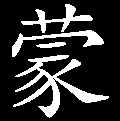
\includegraphics[width=3mm]{../Images/00006}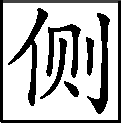
\includegraphics[width=3mm]{../Images/00011}\footnotesize \kaishu 真疼真爱、真怜真惜中,每每生出此等心病来。}这病也不得一日重似一日。''

林黛玉听了这话,如轰雷掣电,细细思之,竟比自己肺腑中掏出来的还觉恳切,{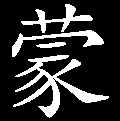
\includegraphics[width=3mm]{../Images/00006}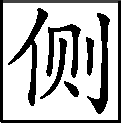
\includegraphics[width=3mm]{../Images/00011}\footnotesize \kaishu 何等神佛开慧眼,照见众生业障,为现此锦绣文章,说此上乘功德法。}竟有万句言语,满心要说,只是半个字也不能吐,却怔怔的望着他。此时宝玉心中也有万句言语,不知从那一句上说起,却也怔怔的望着黛玉。两个人怔了半天,林黛玉只``咳''了一声,两眼不觉滚下泪来,回身便要走。{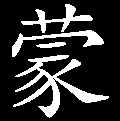
\includegraphics[width=3mm]{../Images/00006}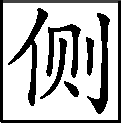
\includegraphics[width=3mm]{../Images/00011}\footnotesize \kaishu 下笔时用一``走'',文之大力,孟贲不若也。}宝玉忙上前拉住,说道:``好妹妹,且略站住,我说一句话再走。''林黛玉一面拭泪,一面将手推开,说道:``有什么可说的。你的话我早知道了!''口里说着,却头也不回竟去了。

宝玉站着,只管发起呆来。{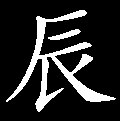
\includegraphics[width=3mm]{../Images/00009}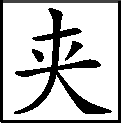
\includegraphics[width=3mm]{../Images/00012}\footnotesize \kaishu 儿女之情毕露,至此极矣!}原来方才出来慌忙,不曾带得扇子,袭人怕他热,忙拿了扇子赶来送与他,忽抬头见了林黛玉和他站着。一时黛玉走了,他还站着不动,因而赶上来说道:``你也不带了扇子去,亏我看见,赶了送来。''宝玉出了神,见袭人和他说话,并未看出是何人来,便一把拉住,说道:``好妹妹,我的这心事,从来也不敢说,今儿我大胆说出来,死也甘心!我为你也弄了一身的病在这里,又不敢告诉人,只好掩着。只等你的病好了,只怕我的病才得好呢。睡里梦里也忘不了你!''袭人听了这话,吓得魄消魂散,只叫``神天菩萨,坑死我了!''便推他道:``这是那里的话!敢是中了邪?还不快去?''宝玉一时醒过来,方知是袭人送扇子来,羞的满面紫涨,夺了扇子,便忙忙的抽身跑了。

这里袭人见他去了,自思方才之言,一定是因黛玉而起,如此看来,将来难免不才之事,令人可惊可畏。想到此间,也不觉怔怔的滴下泪来,心下暗度如何处治方免此丑祸。正裁疑间,忽有宝钗从那边走来,笑道:``大毒日头地下,出什么神呢?''袭人见问,忙笑道:``那边两个雀儿打架,倒也好玩,我就看住了。''宝钗道:``宝兄弟这会子穿了衣服,忙忙的那去了?我才看见走过去,倒要叫住问他呢。他如今说话越发没了经纬,我故此没叫他了,由他过去罢。''袭人道:``老爷叫他出去。''宝钗听了,忙道:``嗳哟!这么黄天暑热的,叫他做什么!别是想起什么来生了气,{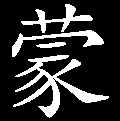
\includegraphics[width=3mm]{../Images/00006}\includegraphics[width=3mm]{../Images/00011}\footnotesize \kaishu 偏是近。}叫出去教训一场。''袭人笑道:``不是这个,想是有客要会。''宝钗笑道:``这个客也没意思,这么热天,不在家里凉快,还跑些什么!''袭人笑道:``倒是你说说罢。''

宝钗因而问道:``云丫头在你们家做什么呢?''袭人笑道:``才说了一会子闲话。你瞧,我前儿粘的那双鞋,明儿叫他做去。''宝钗听见这话,便两边回头,看无人来往,便笑道:``你这么个明白人,怎么一时半刻的就不会体谅人情。我近来看着云丫头神情,再风里言风里语的听起来,那云丫头在家里竟一点儿作不得主。他们家嫌费用大,竟不用那些针线上的人,差不多的东西多是他们娘儿们动手。为什么这几次他来了,他和我说话儿,见没人在跟前,他就说家里累的很。我再问他两句家常过日子的话,他就连眼圈儿都红了,口里含含糊糊待说不说的。想其形景来,自然从小儿没爹娘的苦。{\includegraphics[width=3mm]{../Images/00006}\includegraphics[width=3mm]{../Images/00011}\footnotesize \kaishu 真是知己,不枉湘云前言。}我看着他,也不觉的伤起心来。''袭人见说这话,将手一拍,说:``是了,是了。怪道上月我烦他打十根蝴蝶结子,过了那些日子才打发人送来,还说`打的粗,且在别处能着使罢;要匀净的,等明儿来住着再好生打罢'。如今听宝姑娘这话,想来我们烦他他不好推辞,不知他在家里怎么三更半夜的做呢。可是我也糊涂了,早知是这样,我也不烦他了。''宝钗道:``上次他就告诉我,在家里做活做到三更天,若是替别人做一点半点,他家的那些奶奶太太们还不受用呢。''袭人道:``偏生我们那个牛心左性的小爷,{\includegraphics[width=3mm]{../Images/00006}\includegraphics[width=3mm]{../Images/00011}\footnotesize \kaishu 多情的常有这样``牛心左性''之癖。}凭着小的大的活计,一概不要家里这些活计上的人作。我又弄不开这些。''宝钗笑道:``你理他呢!只管叫人做去,只说是你做的就是了。''袭人笑道:``那里哄的信他,他才是认得出来呢。说不得我只好慢慢的累去罢了。''{\includegraphics[width=3mm]{../Images/00006}\includegraphics[width=3mm]{../Images/00011}\footnotesize \kaishu 痴心的情愿。}宝钗笑道:``你不必忙,我替你作些如何?''袭人笑道:``当真的这样,就是我的福了。晚上我亲自送过来。''

一句话未了,忽见一个老婆子忙忙走来,说道:``这是那里说起!金钏儿姑娘好好的投井死了!''袭人唬了一跳,忙问:``那个金钏儿?''那老婆子道:``那里还有两个金钏儿呢?就是太太屋里的。前儿不知为什么撵他出去,在家里哭天哭地的,也都不理会他,谁知找他不见了。刚才打水的人在那东南角上井里打水,见一个尸首,赶着叫人打捞起来,谁知是他。他们家里还只管乱着要救活,那里中用了!''宝钗道:``这也奇了。''袭人听说,点头赞叹,想素日同气之情,不觉流下泪来。{\includegraphics[width=3mm]{../Images/00006}\includegraphics[width=3mm]{../Images/00011}\footnotesize \kaishu 又一哭法。}宝钗听见这话,忙向王夫人处来道安慰。这里袭人回去不提。

却说宝钗来至王夫人处,只见鸦雀无闻,独有王夫人在里间房内坐着垂泪。{\includegraphics[width=3mm]{../Images/00006}\includegraphics[width=3mm]{../Images/00011}\footnotesize \kaishu 又一哭法。}宝钗便不好提这事,只得一旁坐了。王夫人便问:``你从那里来?''宝钗道:``从园里来。''王夫人道:``你从园里来,可见你宝兄弟?''{\includegraphics[width=3mm]{../Images/00006}\includegraphics[width=3mm]{../Images/00011}\footnotesize \kaishu 世人多是凡事欲瞒人,偏不意中将要着逗露,理之所无而事则多有,何也?}宝钗道:``才倒看见了。他穿了衣服出去了,不知那里去。''

王夫人点头哭道:``你可知道一桩奇事?金钏儿忽然投井死了!''宝钗见说,道:``怎么好好的投井?这也奇了。''王夫人道:``原是前儿他把我一件东西弄坏了,我一时生气,打了他几下,撵了他下去。我只说气他两天,还叫他上来,谁知他这么气性大,就投井死了。岂不是我的罪过。''宝钗叹道:``姨娘是慈善人,固然这么想。据我看来,他并不是赌气投井。多半他下去住着,或是在井跟前憨顽,失了脚掉下去的。他在上头拘束惯了,这一出去,自然要到各处去顽顽逛逛,岂有这样大气的理!纵然有这样大气,也不过是个糊涂人,也不为可惜。{\includegraphics[width=3mm]{../Images/00006}\includegraphics[width=3mm]{../Images/00011}\footnotesize \kaishu 善劝人,大见解!惜乎不知其情,虽精{[}金{]}美玉之言,不中奈何!}''王夫人点头叹道:``这话虽然如此说,到底我心不安。''宝钗叹道:``姨娘也不必念念于兹,十分过不去,不过多赏他几两银子发送他,也就尽主仆之情了。''

王夫人道:``刚才我赏了他娘五十两银子,原要还把你妹妹们的新衣服拿两套给他妆裹。谁知凤丫头说可巧都没什么新做的衣服,只有你林妹妹作生日的两套。我想你林妹妹那个孩子素日是个有心的,况且他也三灾八难的,既说了给他过生日,这会子又给人妆裹去,岂不忌讳。因为这么样,我现叫裁缝赶两套给他。要是别的丫头,赏他几两银子也就完了,只是金钏儿虽然是个丫头,素日在我跟前比我的女儿也差不多。''口里说着,不觉泪下。宝钗忙道:``姨娘这会子又何用叫裁缝赶去,我前儿倒做了两套,拿来给他岂不省事。况且他活着的时候也穿过我的旧衣服,身量又相对。''王夫人道:``虽然这样,难道你不忌讳?''宝钗笑道:``姨娘放心,我从来不计较这些。''一面说,一面起身就走。王夫人忙叫了两个人来跟宝姑娘去。

一时宝钗取了衣服回来,只见宝玉在王夫人旁边坐着垂泪。王夫人正才说他,因宝钗来了,却掩了口不说了。{\includegraphics[width=3mm]{../Images/00006}\includegraphics[width=3mm]{../Images/00011}\footnotesize \kaishu 云龙现影法,可爱煞人。}宝钗见此光景,察言观色,早知觉了八分,于是将衣服交割明白。王夫人将他母亲叫来拿了去。再看下回便知。

{\includegraphics[width=3mm]{../Images/00005}总评:世上无情空大地,人间少爱景何穷。其中世界其中了,含笑同归造化功。}

{袭人、湘云、黛玉、宝钗等之爱之哭,各具一心,各具一见。而宝玉、黛玉之痴情痴性,行文如绘,真是现身说法。岂三家村老学究之可能梦见者!不禁炷香再拜!}

{\href{../Text/part0036_split_000.html\#navto_1_a}{①}此诗见于汤显祖《玉茗堂诗》之九,题《江中见月怀达公》。``却''原作``恰''。}
